\subsection{Ma trận nhầm lẫn và đường cong đánh giá}
\label{subsec:6_5_2}
Hàng của ma trận là nhãn thật, cột là nhãn dự đoán; thứ tự lớp là \texttt{<=50K}, \texttt{>50K}. Với quy ước này, hàng thứ nhất lần lượt là TN, FP; hàng thứ hai lần lượt là FN, TP~\cite{sklearn-cm}. Kết quả gồm TN=11.527, FP=908, FN=1.443 và TP=2.403.

\begin{figure}[htbp]
\centering
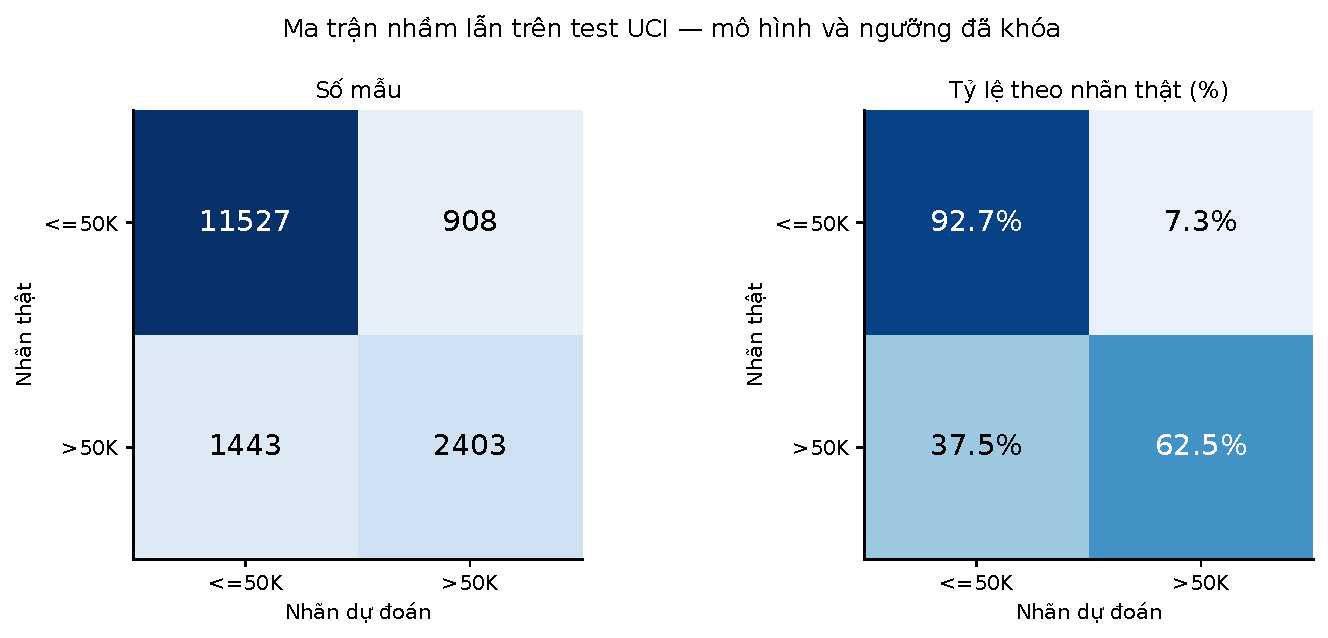
\includegraphics[width=.98\textwidth]{Images/chapter_6/6_5/6_5_2/test_confusion_matrix.pdf}
\caption{Ma trận nhầm lẫn: số mẫu và tỷ lệ chuẩn hóa theo hàng}\label{fig:test-cm}
\end{figure}

\begin{figure}[htbp]
\centering
\begin{minipage}{.49\textwidth}\centering
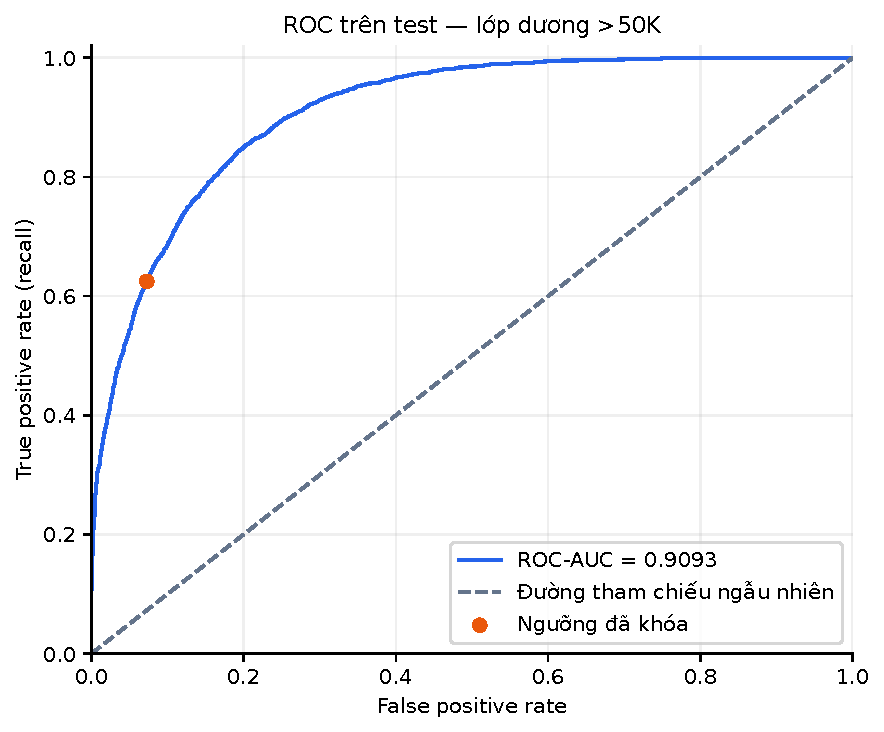
\includegraphics[width=\linewidth]{Images/chapter_6/6_5/6_5_2/test_roc.pdf}
\end{minipage}\hfill
\begin{minipage}{.49\textwidth}\centering
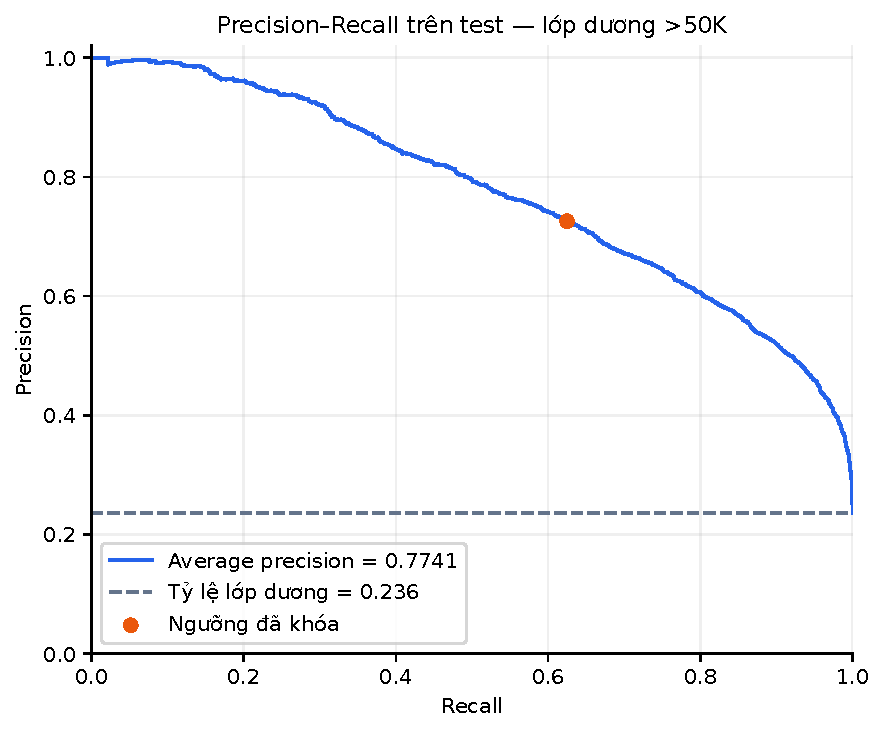
\includegraphics[width=\linewidth]{Images/chapter_6/6_5/6_5_2/test_precision_recall.pdf}
\end{minipage}
\caption{Đường ROC và Precision--Recall trên test; chấm đánh dấu là ngưỡng 0,5 đã khóa}\label{fig:test-curves}
\end{figure}

Mẫu bỏ sót FN chiếm 37,52\% số mẫu dương, trong khi FP chiếm 7,30\% số mẫu âm. Tỷ lệ lớp dương trên test là 23,62\%, được vẽ làm đường tham chiếu trên biểu đồ PR. Các đường cong mô tả sự đánh đổi nếu thay ngưỡng; bài làm giữ nguyên điểm vận hành đã chọn trước khi xem test.
